\subsection{Current State-of-the-Art}
The nature of this project required the visualizations to be rebuilt from the ground up, both to work on the GPU correctly and to synchronize with the concurrent simulation.
This allowed new visualization features to be added.
As a starting point, the supported visualization features of Autodesk CFD 2019 were investigated, and are outlined in \cref{tab:AutodeskCFDSummary}.
This section will explain these features in more detail.

\begin{figure}[ht]
    \centering
    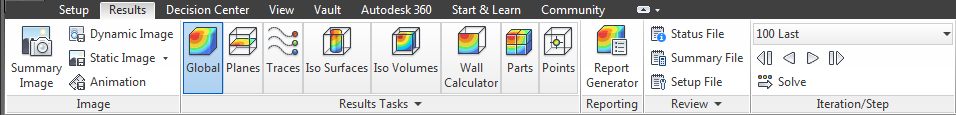
\includegraphics[width=\linewidth]{Ch20Research/figures/results_ribbon.png}
    \caption{Results Ribbon for Autodesk CFD 2019\cite[Results Visualization]{AutodeskCFDManual}}
    \label{fig:AutodeskCFDRibbon}
\end{figure}

\begin{table}[ht]
    \centering
    \begin{tabular}{c|c}
        Tool & Type \\
        \hline
        Global Controls & Visual \\
        Planes & Visual \\
        Iso Surfaces & Visual \\
        Iso Volumes & Visual \\
        Particle Traces & Visual \\
        \hline
        Wall Calculator & Text \\
        Parts & Text \\
        Points & Text \\
    \end{tabular}
    \caption{Summary of results tools from Autodesk CFD.}
    \label{tab:AutodeskCFDSummary}
\end{table}

Autodesk CFD is a 3D simulation/visualization, typically involving one or more 3D surfaces (a 'model') and simulating the fluid movement around these surfaces.
The simulation process creates multiple quantities, including scalar quantities Speed, Temperature, Pressure; and Vector quantities such as Velocity.

\textbf{Global Controls}\cite[Global Controls]{AutodeskCFDManual} visualize selected quantities on all model surfaces.
A scalar quantity can be displayed by changing the surface colour according to a scale (\cref{fig:AutodeskCFDGlobalControlsScalar}).
A vector quantity can be displayed by creating small arrows on the surfaces that represent the direction and magnitude of the quantity.
The range of displayed values can be changed for both the scalar and vector quantities.

A key limitation of this method is it does only shows the quantities on the surface, not the quantities inside the fluid.
Result Planes, Iso Surfaces, and Iso Volumes address this by calculating new surfaces/volumes which visualize quantities.
% These principles extend to most of the other visual tools, which generally define new surfaces to display quantities.

\begin{figure}
    \centering
    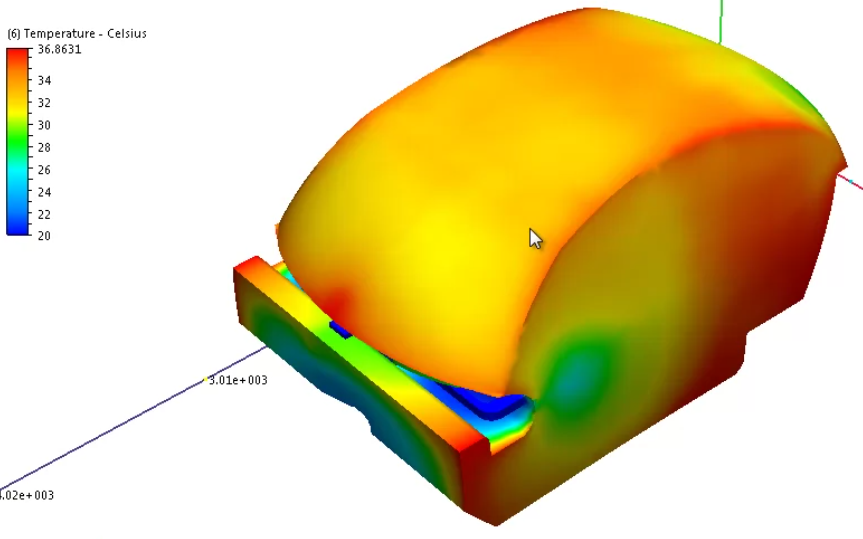
\includegraphics[width=\linewidth]{Ch20Research/figures/autodesk_cfd_global_results_scalar.PNG}
    \caption{Using the Global Controls to visualize a scalar result\cite{AutodeskCFDExercise7}}
    \label{fig:AutodeskCFDGlobalControlsScalar}
\end{figure}

\textbf{Results Planes}\cite[Planes]{AutodeskCFDManual} define a flat cross-section of the model which can visualize a single scalar quantity with a single vector quantity (\cref{fig:AutodeskCFDResultsPlane}).

\begin{figure}
    \centering
    \subcaptionbox{Scalar Quantity}[\linewidth]{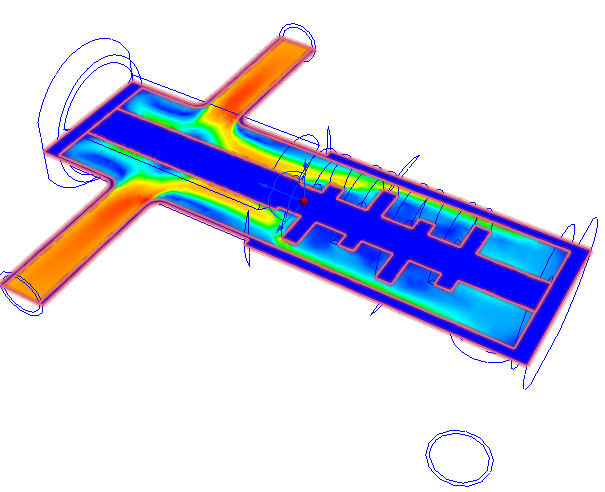
\includegraphics[width=\linewidth]{Ch20Research/figures/autodesk_cfd_results_planes_scalar.png}}
    \subcaptionbox{Vector Quantity}[\linewidth]{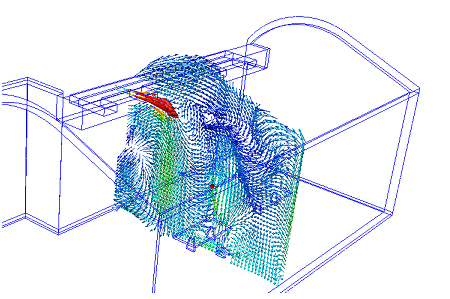
\includegraphics[width=\linewidth]{Ch20Research/figures/autodesk_cfd_results_planes_vector.png}}
    \caption{Result Planes displaying different types of Quantity}
    \label{fig:AutodeskCFDResultsPlane}
\end{figure}

\textbf{Iso surfaces} define a surface based on the value of a result scalar quantity, e.g. $T = \SI{5}{\celsius}$.
This surface can then display a separate scalar and vector quantity, just like a Result Plane (\cref{fig:AutodeskCFDIsosurface}).

\begin{figure}
    \centering
    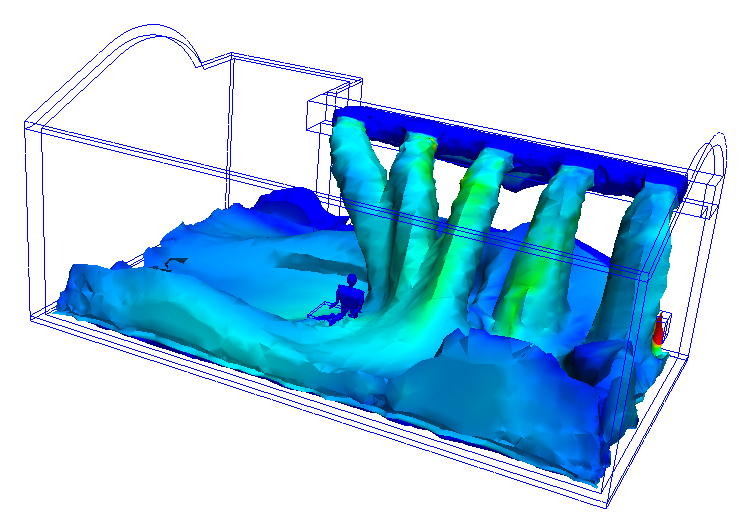
\includegraphics[width=\linewidth]{Ch20Research/figures/isosurface.png}
    \caption{An example of an Isosurface, defined by a velocity magnitude and displaying static pressure.}% ``The iso-surface shape indicates everywhere in the model that has a specific velocity magnitude. The colours indicate the static pressure at these locations.''
    \label{fig:AutodeskCFDIsosurface}
\end{figure}

\textbf{Iso volumes} are similar to an isosurface but define a volume based on a value range ($\SI{0}{\celsius} \leq T \leq \SI{5}{\celsius}$).
A vector quantity can be displayed at points within the volume, and the surface of the volume can show a scalar quantity.


\begin{figure}
    \centering
    \begin{subfigure}{0.45\textwidth}%
        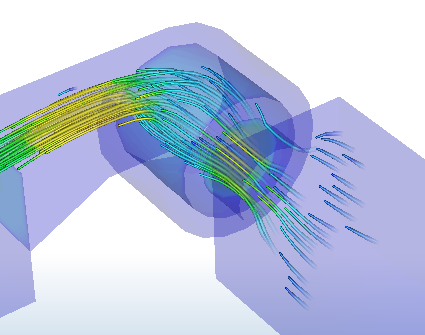
\includegraphics[width=\linewidth]{Ch20Research/figures/autodesk_particle_comets.png}%
        \caption{Particle Comets}%
    \end{subfigure}%
    \begin{subfigure}{0.45\textwidth}%
        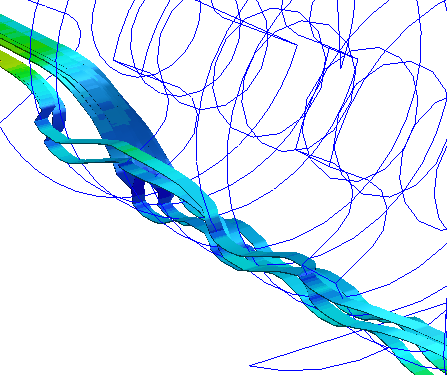
\includegraphics[width=\linewidth]{Ch20Research/figures/autodesk_particle_ribbons.png}%
        \caption{Particle Ribbons}%
    \end{subfigure}
    
    \begin{subfigure}{0.9\textwidth}%
        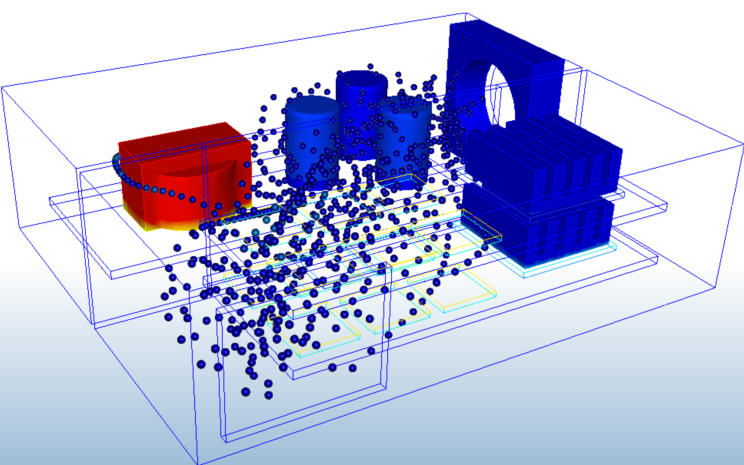
\includegraphics[width=\linewidth]{Ch20Research/figures/autodesk_particle_spheres.jpg}
        \caption{Particle Spheres}
    \end{subfigure}%
    \caption{Examples of Autodesk particle trails.}
    \label{fig:AutodeskCFDParticles}
\end{figure}

\textbf{Particle Traces} show the path particles would take through the flow after being emitted at certain points (or `seeds').
Autodesk allows these paths to be traced forwards or backwards, allows particles to be simulated both with mass and without, and allows a variety of particle trails to be shown (\cref{fig:AutodeskCFDParticles}).

\subsection{Stagnation \& Composition}
The techniques described above have been well known for at least 20 years.
The most prevalent algorithm for computing iso-surfaces was published in 1987\cite{LorensenMarching}.
% Source for marching-cubes being first? is https://www.routledge.com/Isosurfaces-Geometry-Topology-and-Algorithms/Wenger/p/book/9781466570979
Particle Traces and Results Planes were used in 1999\cite{Schulz1999}, although this is not the origin of either technique.
In some cases, there has been extensive research into optimizing visualization techniques\cite{Ueng1996}, and in domain-specific areas there is academic research into creating new techniques\cite{Chen16}, but research into new generic visualization techniques has stagnated.
This stagnation was noted in \cite{vizRole2004} from 2004, which concluded the primary challenges facing visualization were ``identifying and characterizing features'' to visualize rather than developing new techniques.
The MET Office's weather reports demonstrate this principle, and show that composing multiple techniques together can increase information density while remaining easy to understand.

\begin{figure}
    \centering
    \includegraphics[width=\linewidth]{Ch20Research/figures/weather_better.PNG}
    \caption{MET Office weather report\cite{video:MetOfficeTenDayTrend}}
    \label{fig:MetOffice}
\end{figure}

\cref{fig:MetOffice} shows at least three visualization techniques used in the same image, each of which has been filtered to relevant points.
\begin{enumerate}
    \item The large blue, orange, and mauve lines show weather `fronts' moving in, the blue line particularly shows a cold front moving in from the north-east.
    \item The arrows show the wind direction, and only appear in areas with high wind speeds. In the video they also move, making it easier to understand at a glance.
    \item The gray and dark blue shape overlays show cloud cover and rain, respectively.
\end{enumerate}
This proves the potential of combining multiple techniques, which was taken into account when building the program.

\subsection{Realtime Particle Simulation Techniques}\label{sec:Research:Viz:Particles}
The particle simulation element of our visualization doesn't affect the simulation content, and does not have to be completely accurate as long as the flow is approximately correct for the viewer.
That is, the particle movement should fulfil \cref{eq:UnsteadyFlow}\cite{Lane93}
for the following variables:
\begin{itemize}
    \item $p = $ particle position.
    \item $t = $ time, and $t \in [t_1, t_n] \text{where} n = $ number of timesteps.
    \item $\vec{V}(p, t) = $ fluid velocity at point $p$ and time $t$.
\end{itemize}

\begin{figure}
\centering
\[ \frac{dp}{dt} = \vec{V}(p, t) \]

    \caption{Equation for particle movement in unsteady flow.}
    \label{eq:UnsteadyFlow}
\end{figure}
The unsteady-flow variant is shown because the fluid and particles will be moving at the same time, so the fluid itself is unsteady.

A common numerical method for accurately integrating this is the second-order Runge-Kutta scheme with adaptive timesteps, described in \cite{Lane93}.
This takes a constant step size $0 < c \leq 1$ which can be changed to control accuracy.
\begin{multline}
    h = c\norm{\vec{V}(p_k, t)}, \qquad p^{*} = p_k + h\vec{V}(p_k, t), \\
    p_{k+1} = p_k + h\frac{(\vec{V}(p_k, t) + \vec{V}(p^{*}, t + h))}{2}, \\
    t = t + h, \qquad k = k + 1
\end{multline}

A key issue with implementing this method in the program is that $\vec{V}$ is only kept in memory for one value of $t$, so interpolating between $\vec{V}(p_k, t) \text{and} \vec{V}(p^{*}, t + h)$ is impossible.
This also requires an indeterminate amount of steps, and potentially a different amount of steps for each particle, which is not GPU friendly.
Instead, a simpler version was chosen based on the steady-state variant.
At the instant the particle is simulated, the fluid is modelled as steady, and the particle moves with the same timestep taken by the simulation.
To avoid particles stepping over cells entirely, the timestep is subdivided into 4 iterations.

\begin{equation}
    \forall i \in [1..4] \qquad{} p_i = p_{i-1} + \vec{V}(p_{i-1}, t) / 4
\end{equation}
If $p$ does not align with a grid space, $\vec{V}(p)$ is chosen using trilinear interpolation between the closest grid cells as specified in \cite{Lane93}.

In addition to the particle simulation, particles must also be spawned and deleted when necessary.
GPU-based particle simulations are standard in video games, which need to run at high frame rates just like our visualization, so their techniques are a natural fit.
A notable method, which has been adapted for this program, is outlined in \cite{WickedEngineParticles}.
This splits the simulation into three phases:
\begin{enumerate}
    \item The kickoff phase, which determines the amount of new particles to create.
    \item The emission phase, which adds the required amount of new particles to the set by pulling from a queue of inactive particles.
    \item The simulation phase, which updates particle positions, adds dead particles to the inactive queue, and adds alive particles to a render queue.
\end{enumerate}
